\section{Diseño}

\subsection{Núcleo}
El transformador es construido con láminas en forma de E y de I, el transformador se construye con 68 láminas de E y con 66 láminas de I, las cuales al ser acomodadas comprenden una sección transversal de $22 \cdot 38 [mm^{2}]$, la cual es la misma sección transversal de nuestro carrete.
En la figura \ref{fig:T1} se muestra las dimensiones de las laminas E además de la I del nucleo.
\\Como último paso cuando se tienen las vueltas alrededor del carrete, se posicionan las laminas como se muestra en la imagen \ref{fig:T2}. 


\begin{figure}[ht!]
    \centering
    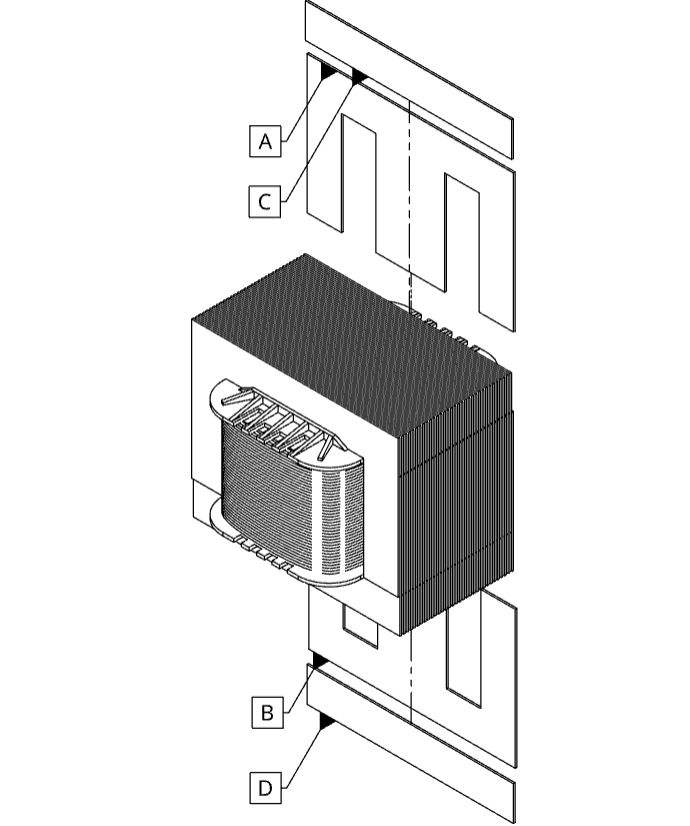
\includegraphics[width=0.48\textwidth]{fot/T2.png}
    \caption{Plano de disposición de las laminas en el nucleo primero se alterna entre el paso A y B sucesivamente hasta que se tenga apretado el carrete y posterior se alterna entre el paso C y D.}
    \label{fig:T2}
\end{figure}



\subsection{Carrete}
El carrete comprende una sección transversal de  $22 \cdot 38 [mm^{2}]$ y una altura de 33 [mm], estos datos son necesarios para poder hacer los cálculos del número de vueltas requeridas para el bobinado primario y el bobinado secundario.
En la figura \ref{fig:T1} se muestra las dimensiones de la sección transversal del carrete.

\begin{figure}[ht!]
    \centering
    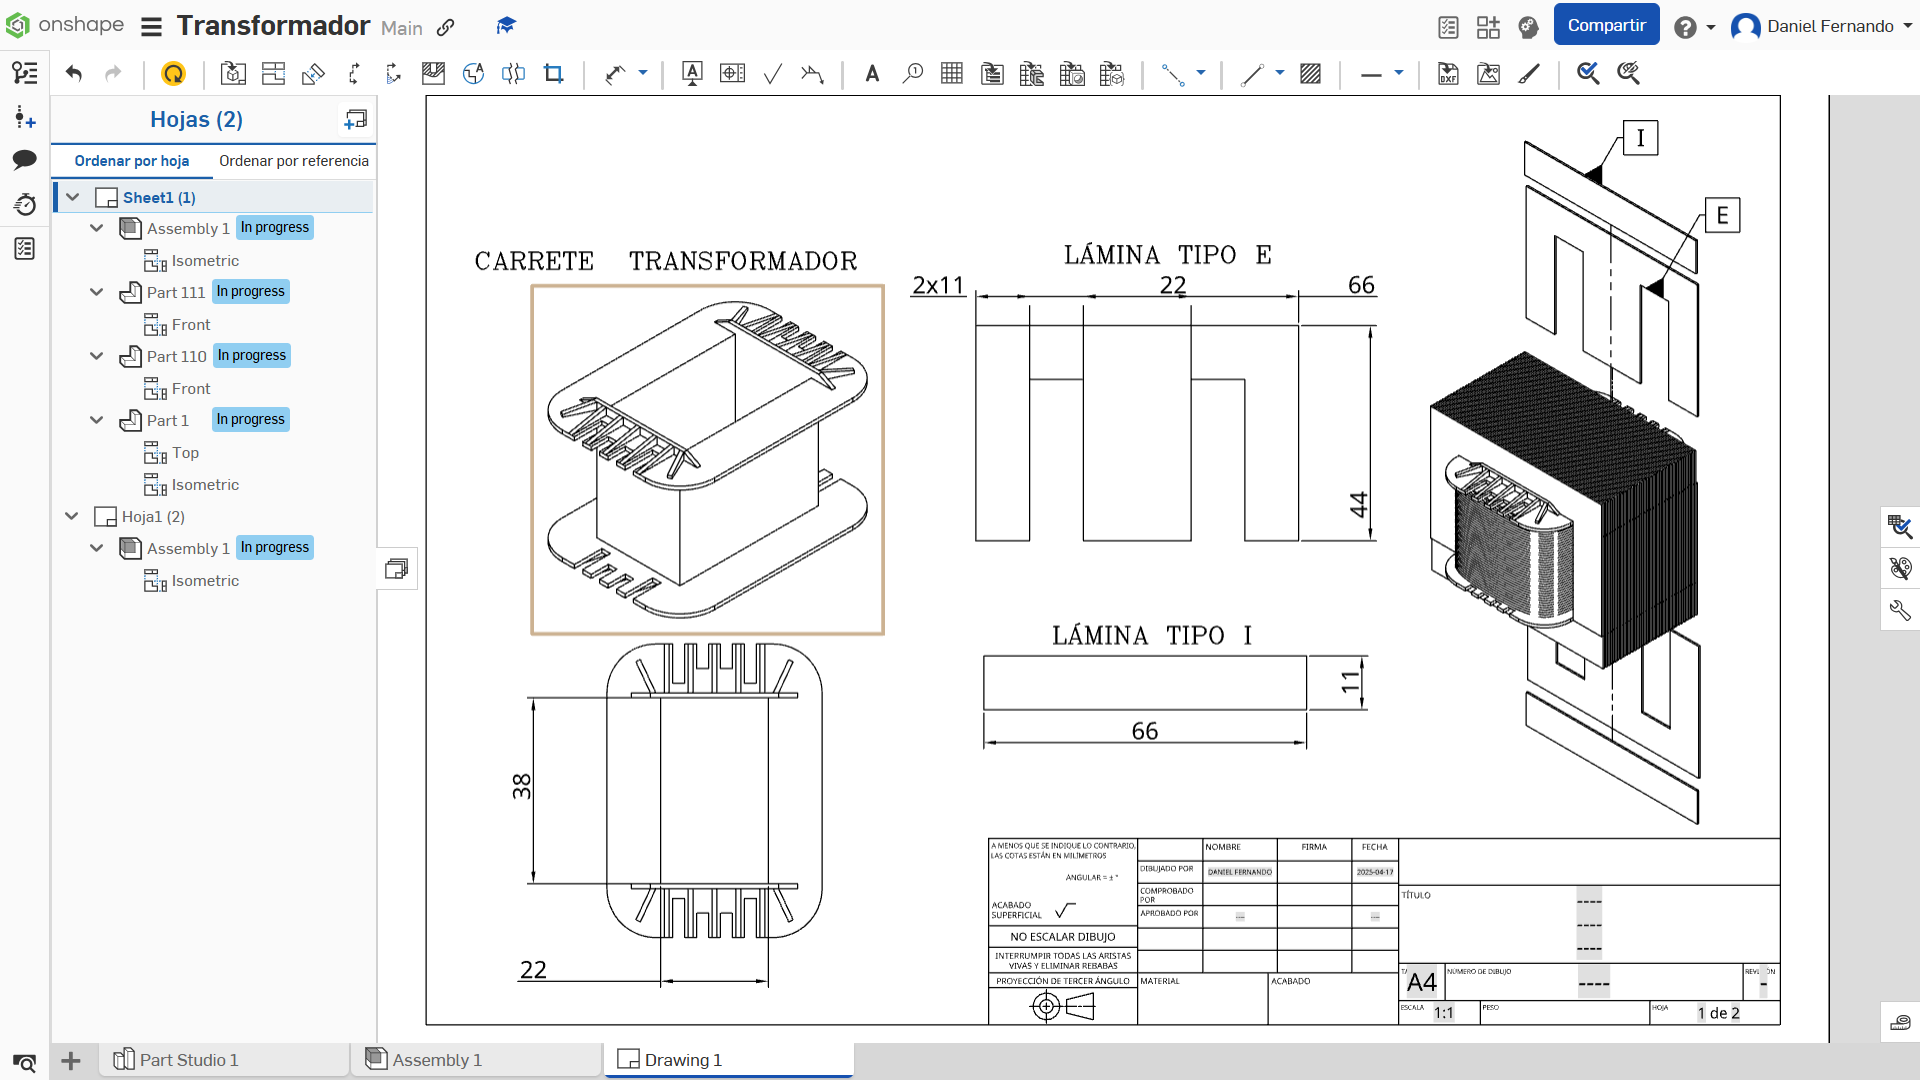
\includegraphics[width=0.48\textwidth]{fot/T1.png}
    \caption{Plano con aspectos constructivos.}
    \label{fig:T1}
\end{figure}



\subsection{Relación de transformación}
Para la relación de transformación elegimos los voltajes de 120 [V] a 50 [V], al realizar la relación de transformación nos queda de la siguiente manera: 

\subsection{Número de vueltas}
\subsection{Bobinado primario}
Teniendo el número de vueltas requerido para el lado primario es de 385, hacemos los cálculos de cuánta corriente podría pasar por el conductor según el voltaje seleccionado 120 [V] y la potencia que queremos 50 [W], seleccionamos un conductor adecuado el cual es cobre esmaltado de calibre --- que permite el paso de una corriente de ---.

\subsection{Bobinado secundario}
Para hallar el número de vueltas que se requiere en el lado secundario lo despejamos de la fórmula de relación de transformación, al aplicarlo tenemos que la cantidad de vueltas será de 160, para este lado secundario también analizamos la corriente que pasará con un voltaje de 50 [V] y una potencia de 50 [W], seleccionamos un conductor de cobre esmaltado de calibre AWG 22 que permite el paso de una corriente de 0.92 A (amperios) a 1.5 A .

\subsection{Aislante}
Se envolvió entre ambos bobinados una capa de papel aislante, el cual ayuda a cubrir ambos bobinados y separarlos entre ellos.

\subsection{Fusibles}
Se agregaron dos fusibles, uno en cada borne de alimentación del transformador, es decir, uno de 2 [A] en el lado de tensión secundario y uno de 5 [A] en el lado de tensión primario, esto para prevenir posibles quemaduras o fallas en el dispositivo.



\begin{figure}[ht!]
    \centering
    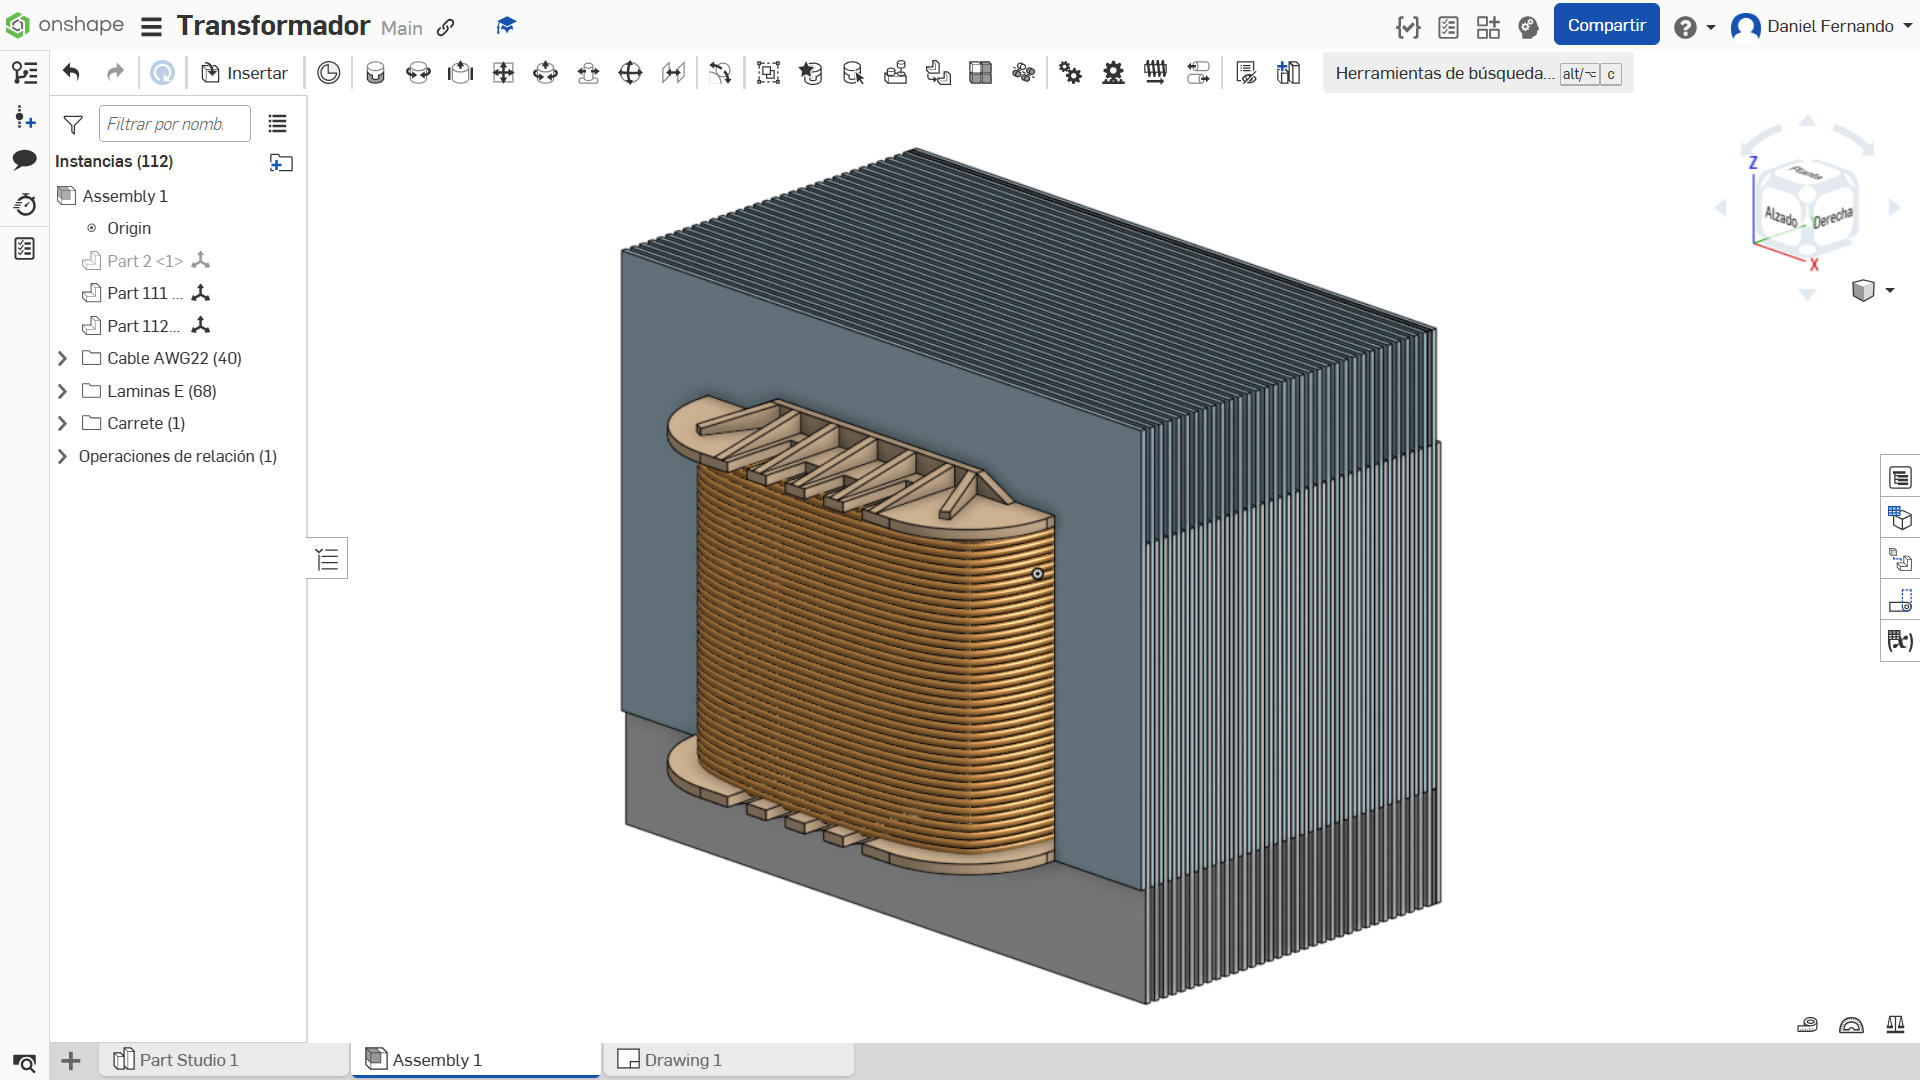
\includegraphics[width=0.48\textwidth]{fot/T3.png}
    \caption{Resultado final del transformador (ocultando los fusibles y el papel aislante).}
    \label{fig:T3}
\end{figure}
